\section*{Selected figures}

\begin{figure}[!ht]
  \centering
  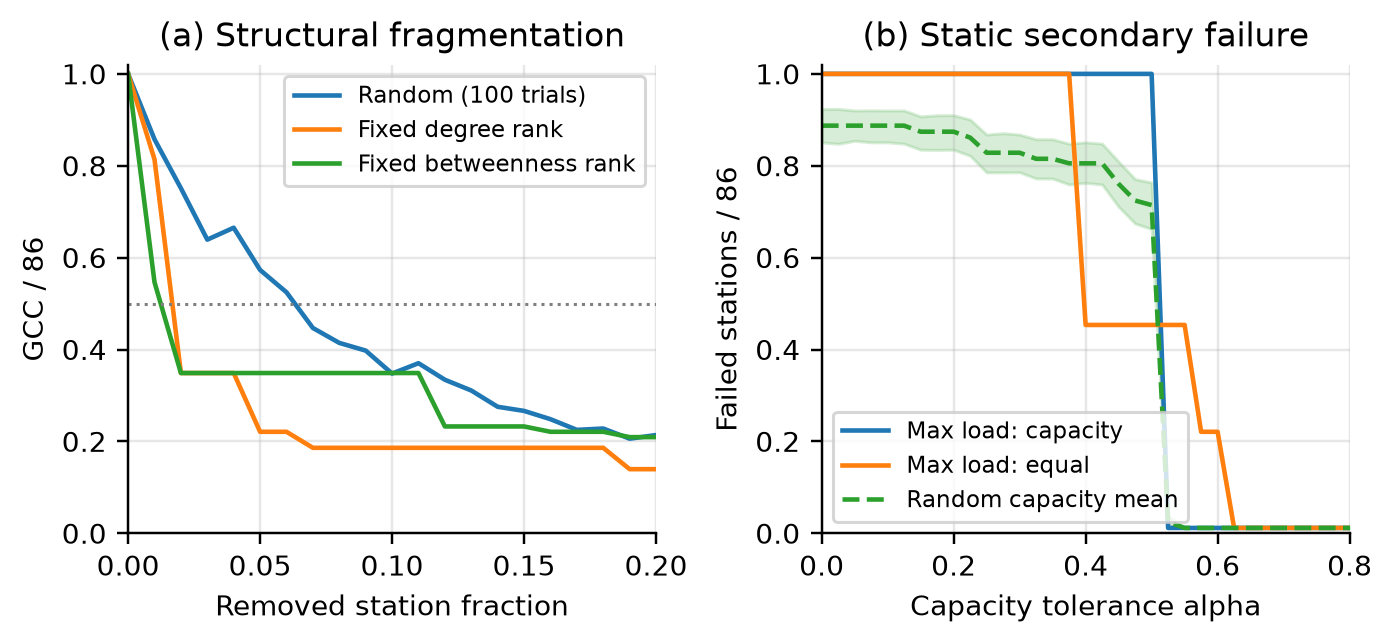
\includegraphics[width=\linewidth]{figures/robustness_cascade.png}
  \caption{Frozen 86-station railway. (a) Station-removal curves, with the
  horizontal GCC/86=0.5 diagnostic. The random mean uses 100 trials per
  fraction; target orders are fixed from the intact graph. (b) Static
  unweighted-betweenness cascades. Targeted curves use the maximum-load station;
  the random capacity-rule mean uses 300 whole trigger trials per alpha and
  pointwise 95\% bootstrap intervals with 2,000 resamples. Failed fractions
  include the trigger. Sources: P2.1 percolation tables, P2.2 runs and P2.5
  cascade intervals; selected by \texttt{report/generate\_figures.py}.}
  \label{fig:robustness-cascade}
\end{figure}

\begin{figure}[!ht]
  \centering
  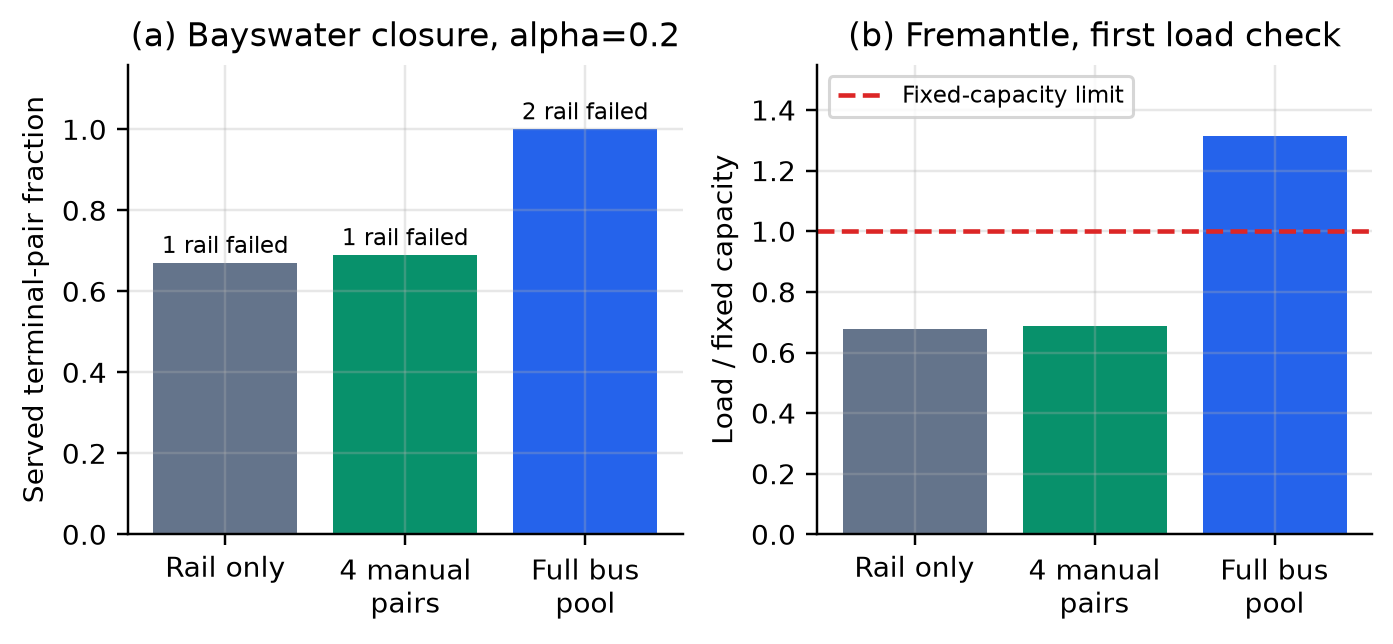
\includegraphics[width=\linewidth]{figures/bus_service_mechanism.png}
  \caption{Bayswater closure at $\alpha=0.2$, layered dynamic routing with
  capacities fixed from the intact rail-only baseline. (a) Served terminal
  pairs over the original 3,655 pairs; annotations count failed rail facilities,
  including the trigger. (b) Fremantle's load/capacity ratio immediately after
  the trigger, before secondary closures. The full bus pool restores all pairs
  while pushing Fremantle above one. This is immediate unlimited standby,
  not a two-link budget. Sources: P2.3 bus-cascade scan and loads tables.}
  \label{fig:bus-mechanism}
\end{figure}

\clearpage
\begin{figure}[!ht]
  \centering
  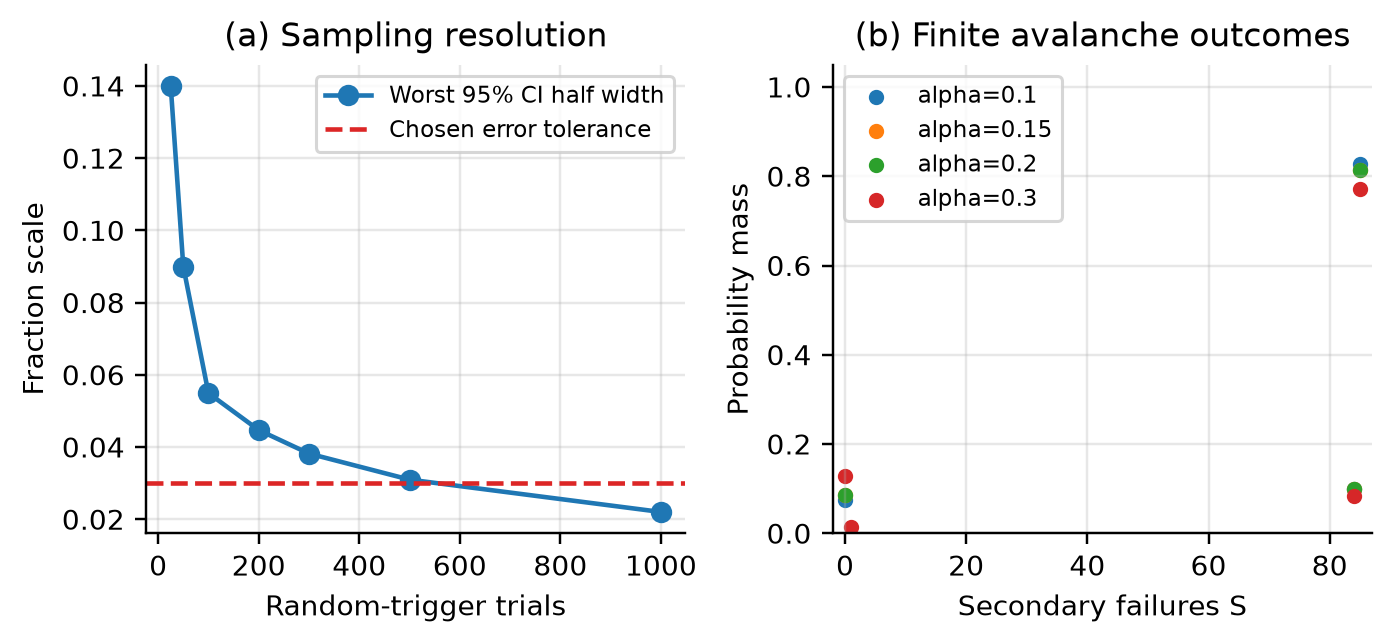
\includegraphics[width=\linewidth]{figures/uncertainty_avalanche.png}
  \caption{Uncertainty is conditional on the frozen graph and load model.
  (a) Worst pointwise 95\% interval half width over the tested conditions with
  a common available prefix size. The 0.03 line is a chosen numerical tolerance;
  the accompanying mean-change criterion is checked separately. (b) Static
  capacity-rule probability masses from 2,000 random triggers at each alpha;
  zero secondary failures remain in the denominator and alphas are not pooled.
  Most mass lies at a few finite sizes, unsuitable evidence for broad scaling.
  Sources: P2.5 recommendations and P2.2 avalanche samples.}
  \label{fig:uncertainty}
\end{figure}
